%------------------------------ EQUATION DERIVATION ------------------------------%
\section{Equation Derivation} \label{app:eq_der}

No additional equation derivation.

%------------------------------ ADDITIONAL ANALYSIS ------------------------------%
\section{Additional Analysis} 
%------------------------------ Coordinate ------------------------------%
\subsection{Robot Coordinate System}
\label{app:coordinate}
For some calculations, the cartesian coordinates are used. Figure \ref{fig:coordinate_system} shows the coordinate system used throughout the report.
\begin{figure}[H]
    \centering
    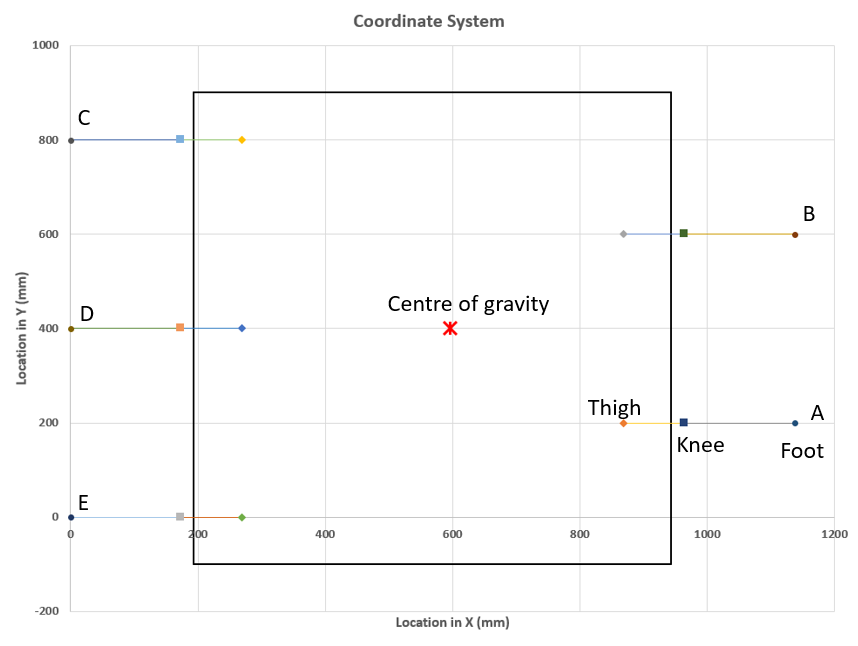
\includegraphics[width=0.8\textwidth]{7_Appendices/Images/CoordinateSystem.PNG}
    \caption{Coordinate System for the robot}
    \label{fig:coordinate_system}
\end{figure}

%------------------------------ Approximation Curved Beam ------------------------------%
\subsection{Approximation Curved Beam}\label{app:approximation_curved_beam}
This is an alternative method to calculating the curved beam stresses due to the complex cross section.

The approximation is to calculate the distance from centroidal axis to neutral axis $e$. The values are obtained from section \ref{subsec:limbs}

\begin{equation}
    e = \frac{I}{r_c A} = \frac{\frac{\pi}{64}((17.175mm)^4 - (14mm)^4)}{(17.175mm)(\frac{\pi}{4}((17.175mm)^2-(14mm)^2)} = 1.79 mm
\end{equation}

\begin{equation}
    c_i = r - e = 8.58mm - 1.79mm = 6.80mm
\end{equation}

\begin{equation}
    \sigma_i = \frac{Mc_i}{Aer_i} = \frac{(20255.6Nmm)(6.8mm)}{(8.59mm)(77.7mm^2)(1.8mm)} = 115.5 MPa
\end{equation}

\begin{equation}
    n = \frac{Sy}{\sigma_i + \sigma_x} = \frac{250 MPa}{115.5 MPa + 1.1 MPa} = 2.2
\end{equation}

%------------------------------ Limbs ------------------------------%
\subsection{Limbs and Internal Stresses}
\label{app:limb_analysis}Only the member BC stress diagram is shown in Section \ref{subsec:limbs}. All three links internal stresses are shown below.

%--- Link AB 
\begin{figure}[H]
    \centering
    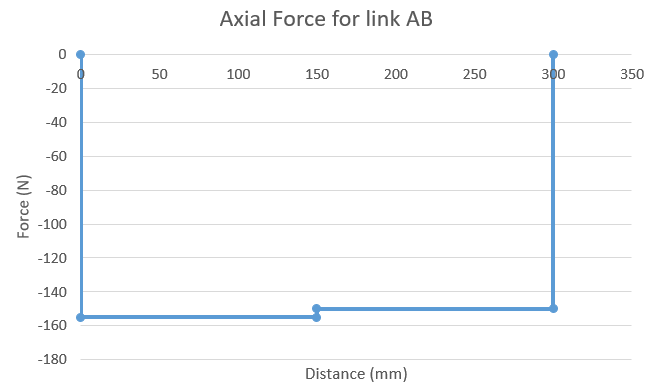
\includegraphics[width=0.8\textwidth]{7_Appendices/Images/AB_Axial.PNG}
    \caption{Axial Force Diagram for link AB}
    \label{fig:annex_limb_AB_axial}
\end{figure}
\begin{figure}[H]
    \centering
    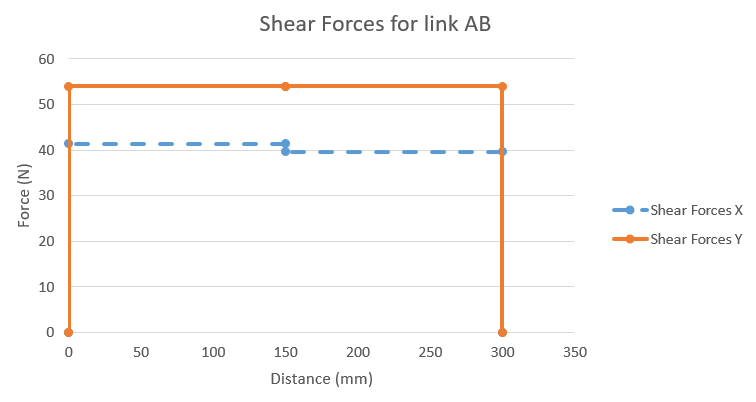
\includegraphics[width=0.8\textwidth]{7_Appendices/Images/AB_Shear.PNG}
    \caption{Shear Force Diagram for link AB}
    \label{fig:annex_limb_AB_shear}
\end{figure}
\begin{figure}[H]
    \centering
    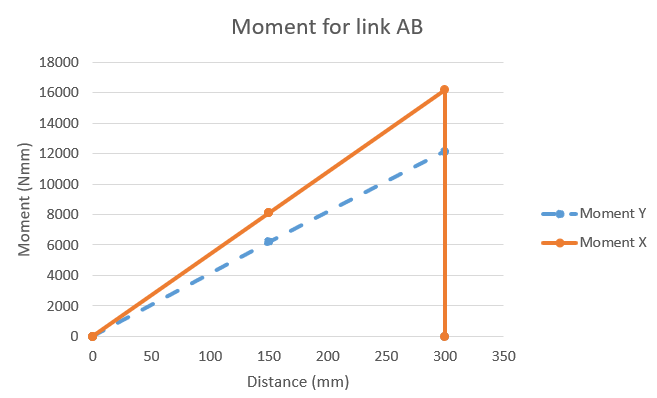
\includegraphics[width=0.8\textwidth]{7_Appendices/Images/AB_Moment.PNG}
    \caption{Moment Diagram for link AB}
    \label{fig:annex_limb_AB_moment}
\end{figure}
%--- Link BC 
\begin{figure}[H]
    \centering
    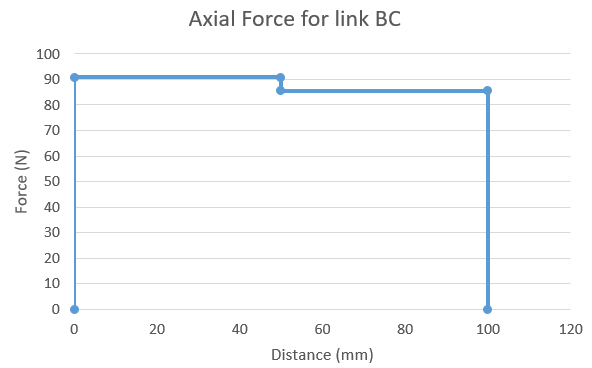
\includegraphics[width=0.7\textwidth]{7_Appendices/Images/BC_Axial.PNG}
    \caption{Axial Force Diagram for link BC}
    \label{fig:annex_limb_BC_axial}
\end{figure}
\begin{figure}[H]
    \centering
    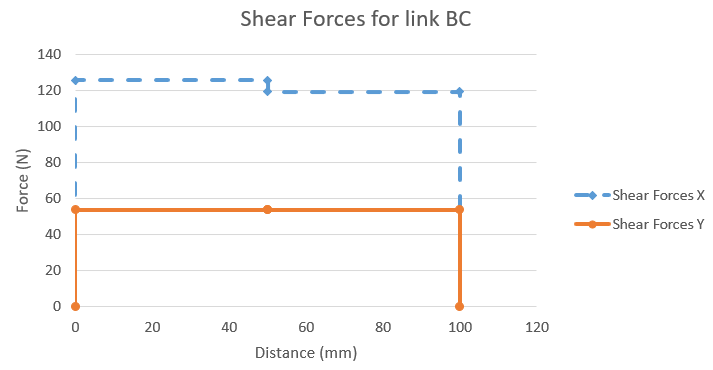
\includegraphics[width=0.8\textwidth]{7_Appendices/Images/BC_Shear.PNG}
    \caption{Shear Force Diagram for link BC}
    \label{fig:annex_limb_BC_shear}
\end{figure}
\begin{figure}[H]
    \centering
    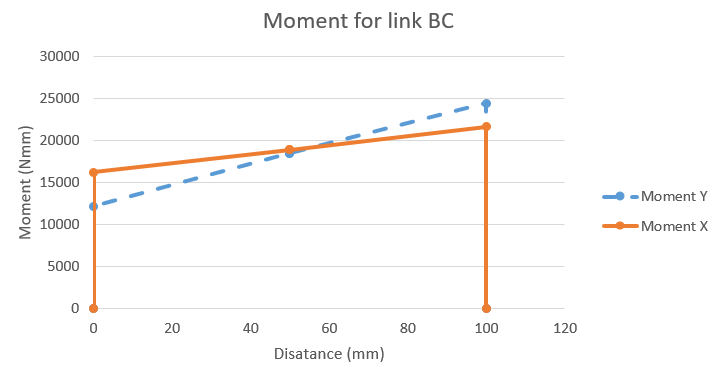
\includegraphics[width=0.8\textwidth]{7_Appendices/Images/BC_Moment.PNG}
    \caption{Moment Diagram for link BC}
    \label{fig:annex_limb_BC_moment}
\end{figure}
%--- Link CD 
\begin{figure}[H]
    \centering
    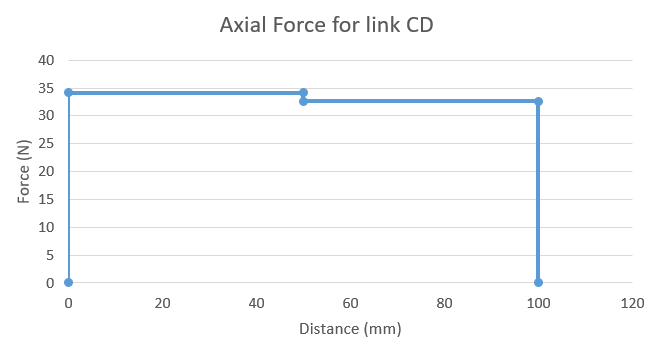
\includegraphics[width=0.8\textwidth]{7_Appendices/Images/CD_Axial.PNG}
    \caption{Axial Force Diagram for link CD}
    \label{fig:annex_limb_CD_axial}
\end{figure}
\begin{figure}[H]
    \centering
    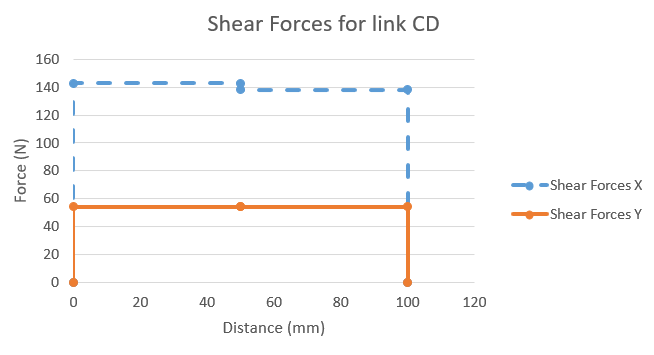
\includegraphics[width=0.8\textwidth]{7_Appendices/Images/CD_Shear.PNG}
    \caption{Shear Force Diagram for link CD}
    \label{fig:annex_limb_CD_shear}
\end{figure}
\begin{figure}[H]
    \centering
    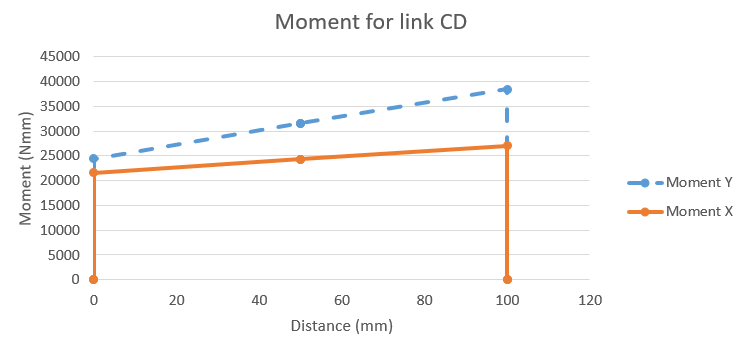
\includegraphics[width=0.7\textwidth]{7_Appendices/Images/CD_Moment.PNG}
    \caption{Moment Diagram for link CD}
    \label{fig:annex_limb_CD_moment}
\end{figure}


\subsection{Ball Bearings} \label{app:ball_bearing}

Originally it was decided to use ball or roller bearings for the shafts in order to limit friction. However, as this application is mostly static, reasonably sized bearings were unable to resist the static radial forces and thus sleeve bearings (bushings) were selected instead. The following equation was used to calculate the required rated capacity $C_{req}$ of the ball bearings \cite{juvinall_fundamentals_2012}:

\begin{equation}
    C_{req}=F_e K_a( \frac{L}{K_r L_R})^{0.3}  
\end{equation}

where $K_a$ is the application factor, $K_r$ is the reliability factor, $L_R$ is the rated life in revolutions, $L$ is the required life in rpm and $F_e$ is the equivalent force, which is dependant on the ratio of axial to radial forces. As an example the value for required rated capacity is calculated for the exterior knee shaft. The values of $K_a=1.4$ for light impact and $K_r=1.0$ for 90\% reliability are chosen based on the Juvinall textbook suggestions \cite{juvinall_fundamentals_2012}. A life of 10000 hours is chosen as the application is used intermittently and requires good reliability. Using the maximum speed of 1.6 rpm, we can get the value of $L=960000$ revolutions. The value of $L_R=10^6$ revolutions is chosen to match the value used by the observed manufacturer (NTN Bearings) \cite{ntn_bearing_deep_nodate}. As the radial force on the bearings is much larger than the axial force, we get that $F_e=F_{radial}=1124.1 N$. We can now get the required rated capacity for the bearing:

\begin{equation}
    C_{req}=1124.1 N (1.4)( \frac{960000 rev}{(1.0) (10^6 rev)})^{0.3}= 12.3 kN
\end{equation}

From the NTN bearings catalogue \cite{ntn_bearing_deep_nodate}, a medium load ball bearing of the appropriate size for this shaft (13 mm diameter) can only support about 10.3 kN dynamic and 4.6 kN static load. The dynamic rating could be achievable by increasing the size of the shaft slightly, but the static rating is extremely low and not feasible. This analysis is what led to the selection of sleeve bearings (or bushings).


\subsection{Sleeve Bearing Friction} \label{app:bearing_friction}

As this application is mostly static or at very low speeds, the bushing is submitted to boundary lubrication \cite{juvinall_fundamentals_2012}. An approximation of the friction coefficient was attempted using Petroff's equation \cite{juvinall_fundamentals_2012}:

\begin{equation}
    f=\frac{2\pi ^2\mu n(d/2)}{Pc} \label{eq:bearing_friction}
\end{equation}{}

where $\mu $ is the absolute viscosity in Pa s and $c$ is the clearance between the shaft and bushing in mm. Absolute viscosity values were difficult to find. A conservative estimate was made, using the Temperature-Grade-Viscosity graph provided in the Juvinall textbook \cite{juvinall_fundamentals_2012}. The highest viscosity grade (SAE 70) was chosen, and assumed to be operating at 30 degrees celsius. This temperature is selected as a reasonable temperature that might be found in the bushing on a cold day (with added friction and electronics heat). This gives an absolute viscosity of 1000 mPas, which is a relatively high value and will give a high estimate of the friction. For the clearance in the bushing, it was found that the ratio of the shaft radius and clearance is generally between 500-1000, therefore a ratio of 1000 was selected as worst case scenario \cite{juvinall_fundamentals_2012}. The value of the friction (drag) torque $T_f$ is then found with the following equation \cite{juvinall_fundamentals_2012}, where $F$ is the radial force applied on the bearing.

\begin{equation}
    T_f=fF(d/2) \label{eq:drag_torque}
\end{equation}{}

For a sample calculation on the exterior knee shaft bearings, the bearing friction coefficient is found using Equation \ref{eq:bearing_friction}, with $\mu = 1000mPas$, $c = \frac{d/2}{1000}=0.0065 mm$, $n=1.60 rpm$ and $d=13.0 mm$. The actual value of pressure $P$ must be calculated first using Equation \ref{eq:bearing_pressure}. Then, the drag torque is found using Equation \ref{eq:drag_torque}.

\begin{gather}
    P=\frac{F}{dL} = \frac{1124.1 N}{13.0 mm\times 4.0 mm}\times=21.6 MPa
    \\
    f=\frac{2\pi ^2\mu n(d/2)}{Pc}=\frac{2\pi ^2\times 1Pas\times (1.60/60) rps \times (13.0 mm/2)}{21.6 \times 10^6 Pa \times 0.0065 mm} = 2.4\times 10^{-5}
    \\
    T_f=fF(d/2)=2.4\times 10^{-5}\times 1125.1 N\times(13.0 mm/2)=0.18 Nmm
\end{gather}

The friction does not make sense as it was found that friction coefficients for boundary lubrication should be about 0.05-0.20 \cite{juvinall_fundamentals_2012}. The calculated value is extremely low. This might be due to the fact that the Petroff equation assumes no eccentricity, which would not be the case for boundary lubrication. The rotation speed in this application is also low, which causes the friction coefficient to be very low. 

If the highest value of coefficient of friction in the range is chosen ($f=0.20$), then a drag torque of 1463 Nmm is found, which is less than 5\% of the applied torque. Thus, as our friction coefficient is likely lower, friction can be considered negligible. 

%------------------------------ DATA SHEETS ------------------------------%
\section{Data sheets} \label{app:datasheets}

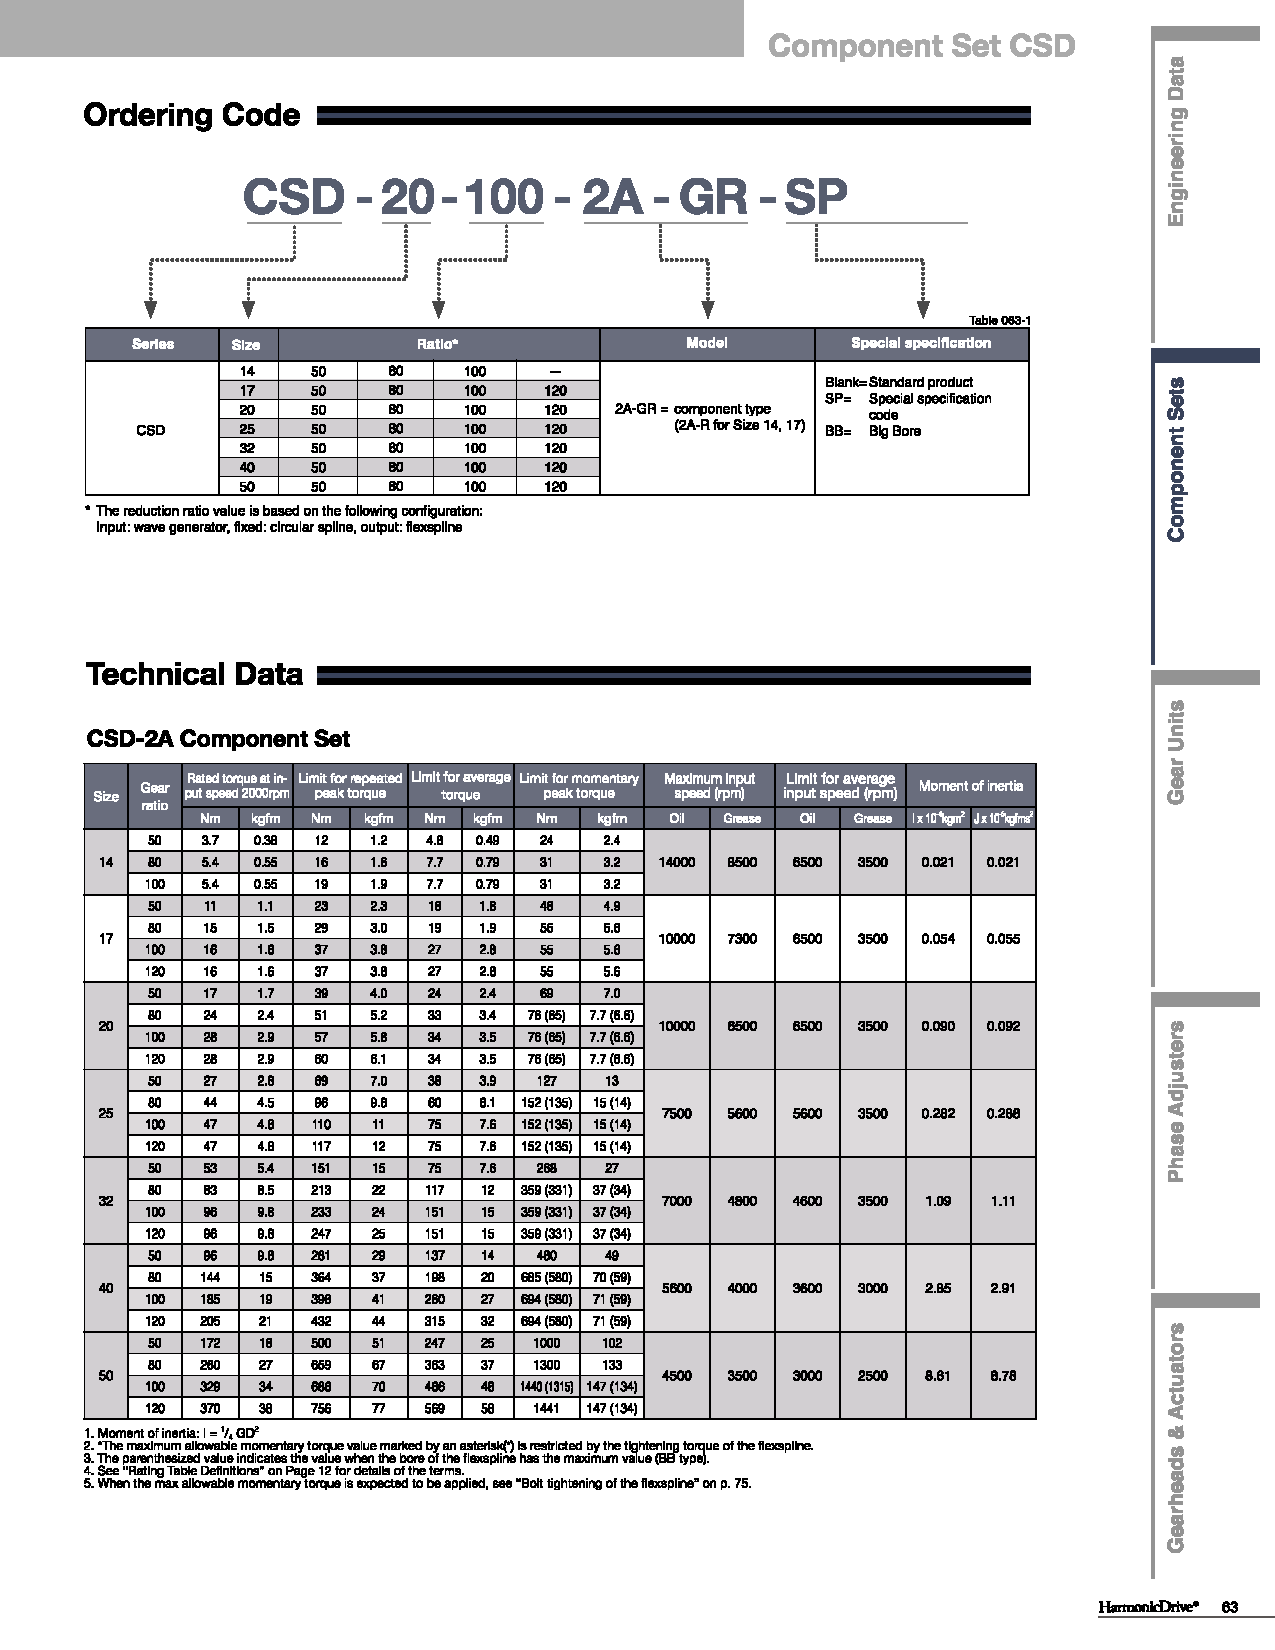
\includepdf[pages=-]{pdf/harmonic_drive_csd.pdf}
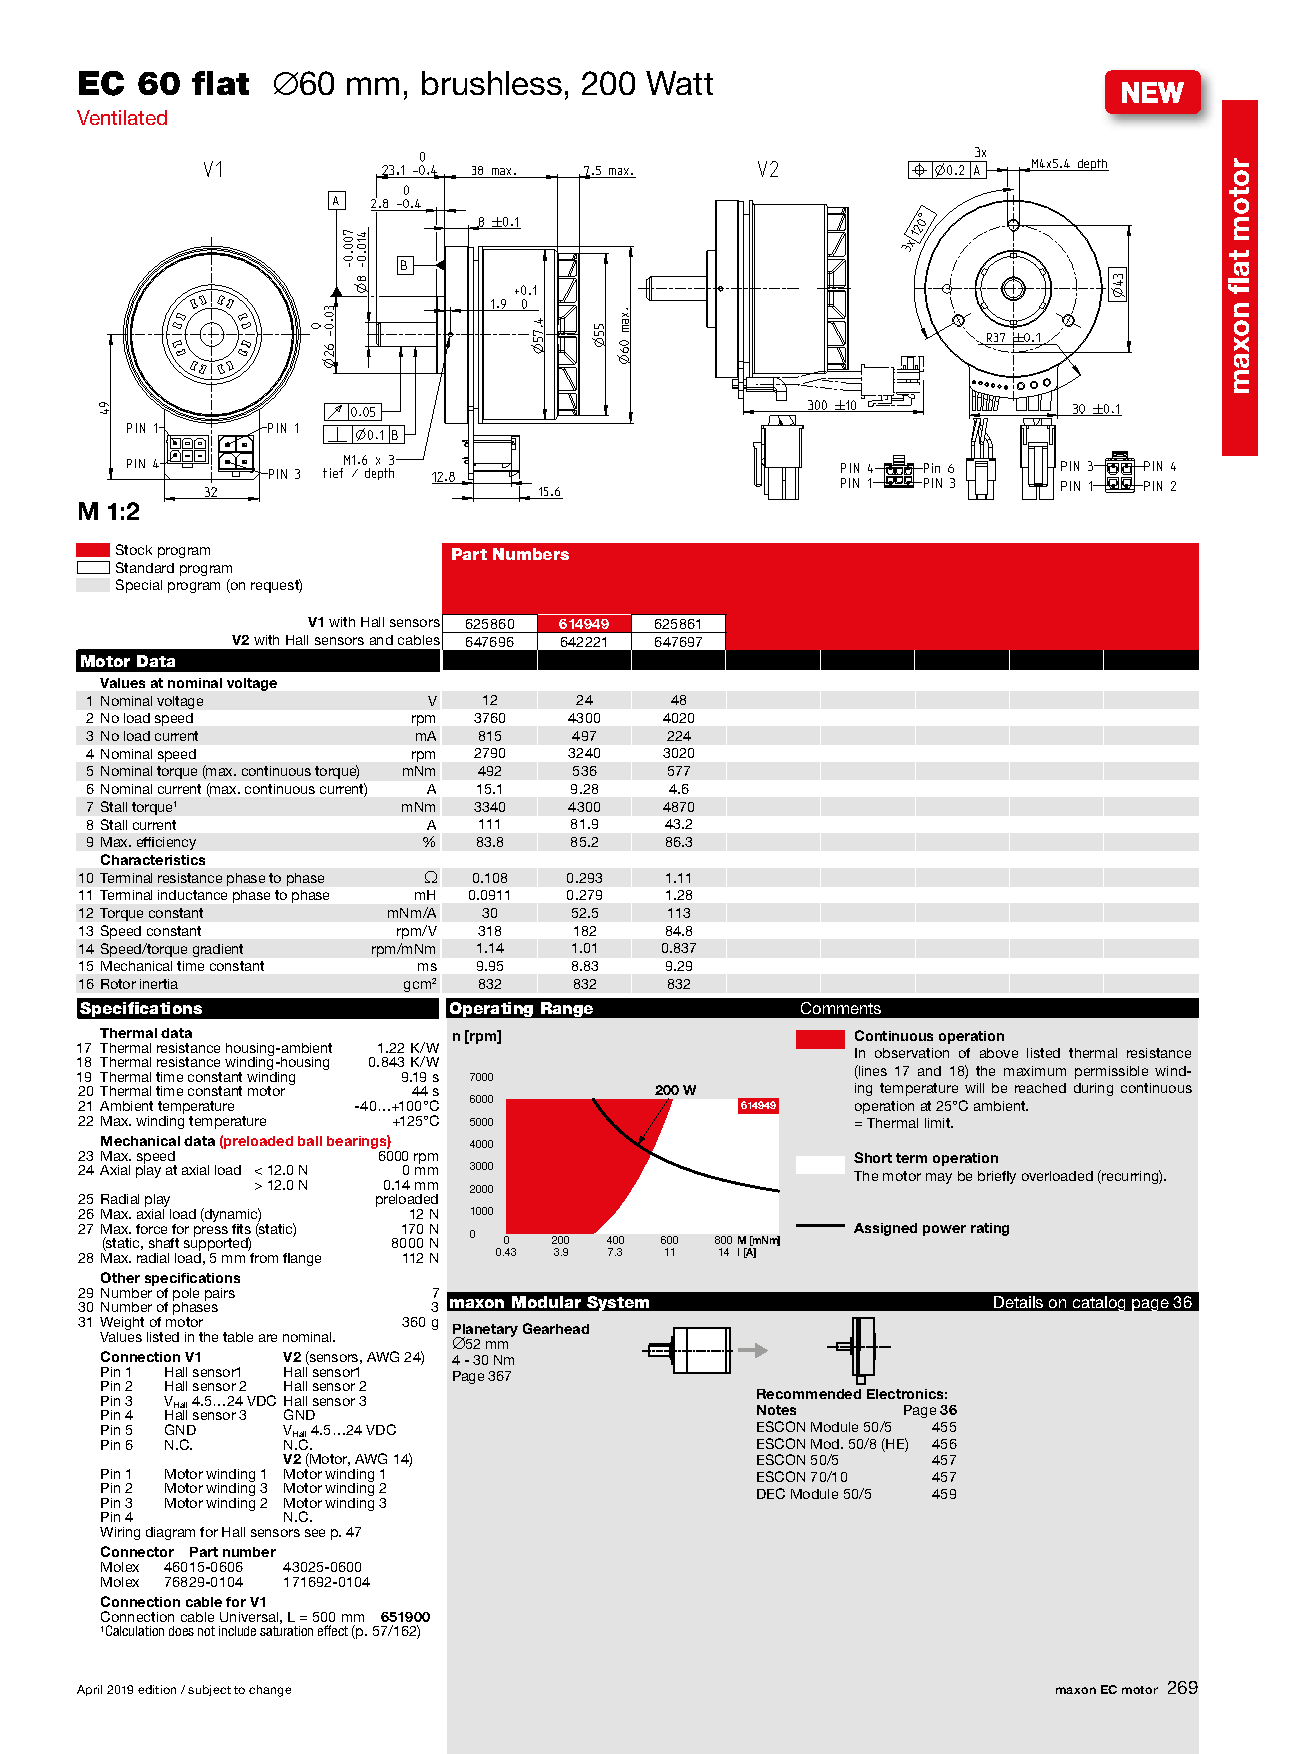
\includepdf[pages=-]{pdf/maxon_ec60_200w.pdf}
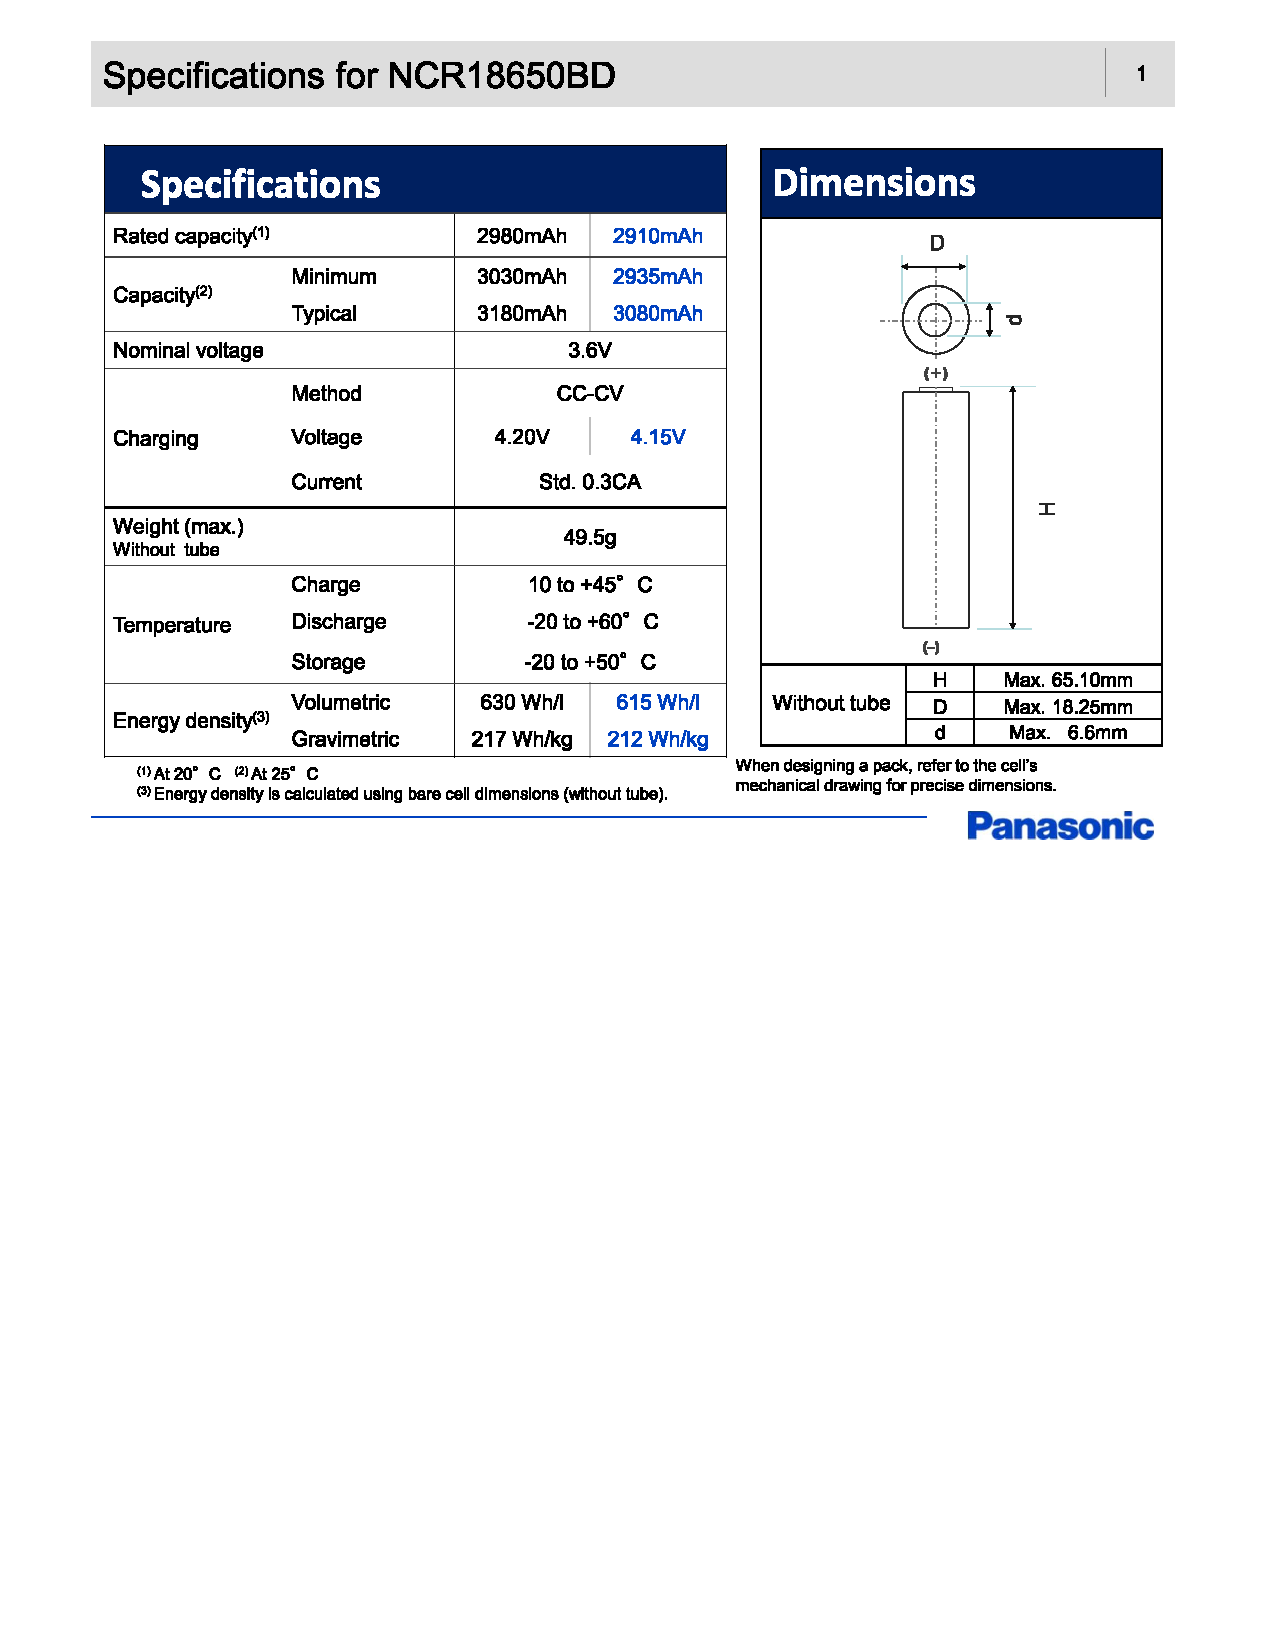
\includepdf[pages=-]{pdf/panasonic_18650.pdf}

\includepdf[pages=-]{pdf/Cell_Solar.pdf}
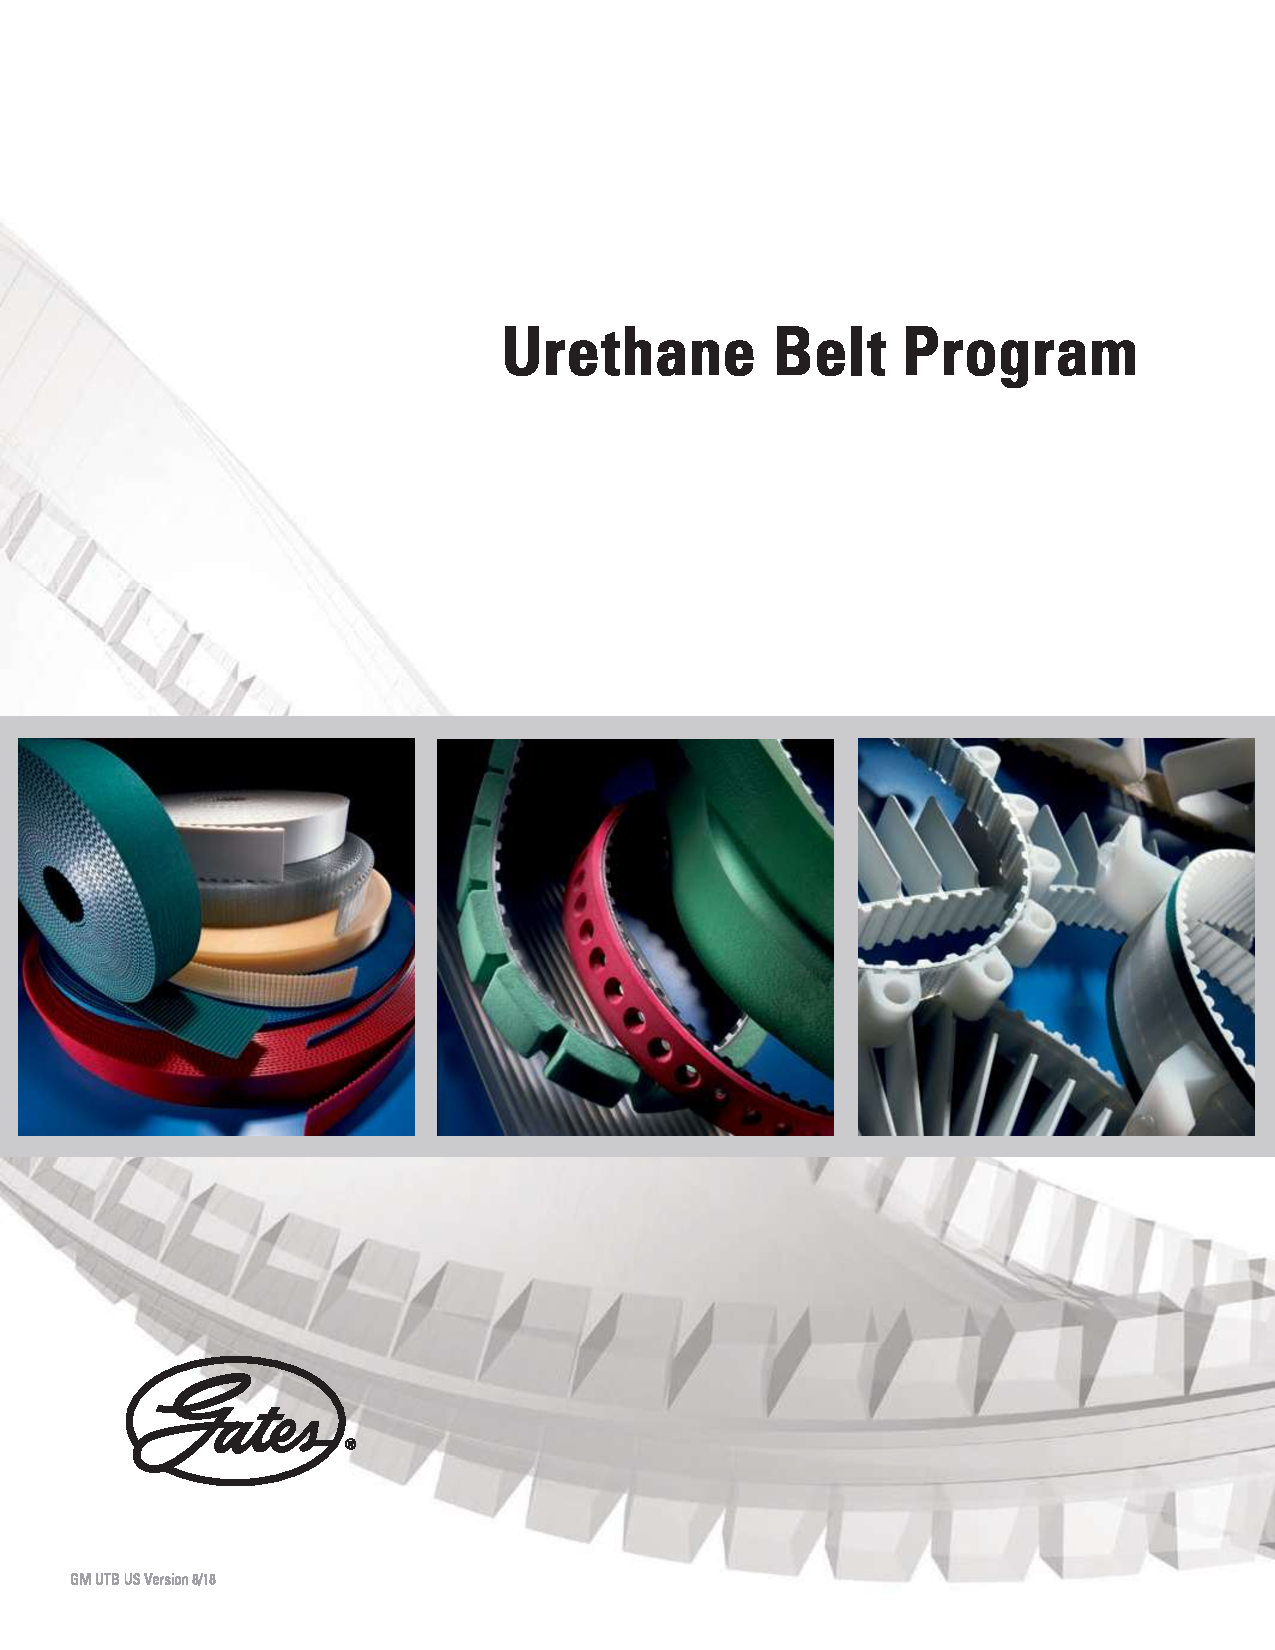
\includepdf[pages=-]{pdf/Condensed_Belt_Catalogue.pdf}


%------------------------------ CODE ------------------------------%
\section{Code} \label{app:code}

\subsection{Power Consumption} \label{app:code_power_consumption}

The power consumption is more accurately calculated using the MATLAB script below.

\subsubsection{Power Consumption Script}

\lstinputlisting[language=Matlab]{Code/PowerConsumption.m}

\subsubsection{Harmonic Drive Inputs Script}

\lstinputlisting[language=Matlab]{Code/HDInputs.m}

\subsubsection{Motor Inputs Script}

\lstinputlisting[language=Matlab]{Code/MotorInputs.m}